\documentclass[12pt,a4paper,oneside]{report}
%\documentclass[12pt,a4paper,twoside,draft]{report}
\usepackage[utf8]{inputenc}
% OLD : \usepackage[utf8x]{inputenc}
\usepackage[english,danish]{babel} 	% dansk orddeling, overskrifter mv.
\usepackage[T1]{fontenc}     		% pæne fonte    
\usepackage{lmodern}				% Bedre fonte til dansk
\usepackage[normalem]{ulem}			% For at kunne tegne en streg over tekst
\usepackage{graphicx}
\usepackage[left=3cm,right=3cm,top=2.5cm,bottom=2.5cm]{geometry}
\usepackage{pdfpages}
\usepackage{fancyhdr}
\usepackage{lastpage}				% Allows determination of last page
\usepackage{mathtools}
\usepackage{amsmath}				% Use math
\usepackage{placeins} 				% Defines \FloatBarrier
\usepackage{mcode} 					% Maa ikke slettes!
\usepackage{listings}				% Latex kode formatering
\usepackage{wrapfig}				% Allow to wrap text and pic
\usepackage{float}
\usepackage{pdfpages}
\usepackage{epstopdf}
\usepackage{url}
\usepackage{multirow}
\usepackage{tabularx}
\usepackage[numbered,framed]{matlab-prettifier}
\usepackage{wasysym}
\usepackage[usenames, dvipsnames]{color}
\usepackage[export]{adjustbox} 		% Vertical allign in subplot

\usepackage{indentfirst}

%\usepackage{mathabx}
\usepackage{graphicx}

\usepackage[hidelinks]{hyperref}
\setcounter{tocdepth}{3}
\usepackage[toc,page]{appendix}
\setcounter{secnumdepth}{3}
\usepackage{color, colortbl}
%\definecolor{name}{system}{definition}
\definecolor{Tab}{gray}{0.9}
\definecolor{Gray}{rgb}{1,0.76,0.76}
\def\emptyline{\vspace{12pt}}
\newcommand{\hilight}[1]{\colorbox{red}{#1}}
\let\conjugatet\overline


\newcommand{\Conv}{\mathop{\scalebox{1.5}{\raisebox{-0.2ex}{$\ast$}}}}%


%% FOR vectors:
\newcount\colveccount
\newcommand*\colvec[1]{
        \global\colveccount#1
        \begin{pmatrix}
        \colvecnext
}
\def\colvecnext#1{
        #1
        \global\advance\colveccount-1
        \ifnum\colveccount>0
                \\
                \expandafter\colvecnext
        \else
                \end{pmatrix}
        \fi
}
%% For vector arrows:

    \newcommand*{\vv}[1]{\vec{\mkern0mu#1}}



%\usepackage{draftwatermark}
\usepackage{subcaption}
\usepackage{amsfonts}
\usepackage{amssymb}
%\usepackage{subfigure}

%\selectlanguage{danish}


\setlength{\headheight}{15pt}
\pagestyle{fancyplain}	% "fancy" -> not header on chapters 
\fancyhead{}		% resets header and footer from default
\fancyfoot{}
\fancyhead[C]{}
\fancyhead[LO,L]{Data Security in Vehicular Networks for Traffic Management}
\fancyhead[RO,R]{Data Security}
%\fancyfoot[C]{\thepage}   % get pagenumber on all pages in "fancy"-style
\fancyfoot[RO,R]{Page \thepage \ of \pageref{LastPage}}

%\parindent = 0pt

% Added command for blue-colored text
\newcommand{\Bluey}[1]{\textcolor{blue}{#1}}

\begin{document}

%\lstset{language=Matlab} 	% Sørger for at bruge matlab highlights
\begin{titlepage}

\begin{center}


\begin{figure}
      \centering
      \begin{minipage}{0.5\linewidth}
          	\raggedright
              
      \end{minipage}
      \begin{minipage}{0.5\linewidth}
          	\raggedleft
              
      \end{minipage}
\end{figure}

\begin{figure}
\centering
\begin{minipage}{1\textwidth}
  \raggedleft
  
\includegraphics[height=17mm]{graphics/frontpage/DTUlogo.png}
\end{minipage}
\end{figure}



\hfill \\[2.5cm]

\textsc{\LARGE Extreme Climate And Physical Nature}\\[0.3cm]

\textsc{\LARGE Course 11857}\\[2cm]

\textsc{\Huge Individual Assignment}\\[3cm]



\hfill \\[4cm]
\textsc{\Large Galina Jonat, s172118 }\\[0.5cm]
\textsc{\Large February/March 2017}\\[0.2cm]


\end{center}
\vfill


\end{titlepage}

\urlstyle{same}
\selectlanguage{english}

\newpage

\renewcommand*{\thesection}{\arabic{section}}

\tableofcontents



%\include{tex/WorkProgress}

\section{Q1: State of the art in Climate Change - Sea Ice}

\subsection{Sea Ice and Climate Change}
Sea Ice is the ice that forms, grows and melts in the ocean. It is floating on the surface and its movement is determined by winds and currents. The average thickness of sea ice is 3 metres; however, the range is between mm-range and 10 metres thickness. Its extent expands and contracts remarkably from winter to summer. When the ice sheet is formed, it does not take in all the salt, which then affects the movement of ocean waters, if it happens in a large scale.
Compared to other Earth surfaces, e.g. the Ocean, Sea Ice has a very high albedo (1), reflecting the Sun’s radiation almost entirely.
Sea Ice is interesting looking at its extent, thickness, concentration, drift and snow thickness above the ice (influencing the albedo). To measure these components, one needs to carry out both remote  sensing measurements and in situ (ground-based) measurements, setting up ice camps (what they used to do a lot earlier), or by using icebreaker ships. The remote sensing “methods” are visible, infrared, active and passive microwave.
Looking at the Sea Ice extent, it has declined rapidly within the past 30 years, showing a minimizing of 13.2 per cent per decade.
This leads to the following changes in the climate and especially the marine system:
\begin{itemize}
    \item Fresher ocean water
    \item More evaporation
    \item Warming oceans (due to decreased albedo)
    \item More extreme events, e.g. storms, increased wave height
    \item Coastal erosion
    \item More acidic water due to higher CO2 uptake
	\item Interruption of the thermohaline circulation
\end{itemize}
As these impacts are not only global, it is necessary to try to understand (model) and predict the development of the Sea Ice. To achieve that, there are two different types of model: one is based on statistical data and the other one is a dynamic model, simulating the interaction between the ocean, atmosphere, the land surface and ice. The models are verified and their performance is measured by using given data to predict for a time that we have data for. However, it will be more and more complicated to create reliable models, as the shrinkage of the multi-year ice increases the year-to-year variability, which is hard to account for.\\
The changes of Sea Ice do also imply effects to the anthroposphere and ecosystems:
With the Sea Ice Mass shrinking, some indigenous traditional lifestyles cannot be practised anymore, such as hunting on the sea ice. Coastal erosion does threaten structures. Some ice adapted species may lose their habitats which will lead to a changing range of the arctic species and changing diets. Some positive effects might be cheaper transport in East-Asia, Europe and North America.




\subsection{Feedback from fellow students}
Well-structured Kept the time Nice introduction (new for most of us, good to give definition), caught the attention Part about how measure using Remote Sensing difficult to understand (Galina has a background that we do not have)


\section{}

\subsection{New Terms}
\textbf{Mass balance:} The mass balance of a glacier or ice sheet is the net balance between the mass gained by snow deposition, and the loss of mass by melting (either at the glacier surface or under the floating ice shelves or ice tongues) and calving (production of icebergs). A negative mass balance means that a glacier is losing mass, and, for grounded glaciers and ice sheets, this mass loss directly contributes to sea level rise (the melting of floating ice shelves and ice tongues does not contribute to sea level rise, because of the lower density of ice as compared to water, which determines the floating portion of the ice). \cite{massBalance}


\subsection{Running the Model 1: Cooling Climate}
For a colder climate our model ice sheet becomes bigger, primarily due to less surface melting (accumulation area is larger). The eustatic sea level lowers as well due to the presence of Northern Hemisphere ice sheets, so that the ice sheet can gradually expand horizontally.




\section{Threats}
Real-time technologies, transferring data via a network, are very vulnerable for attacks. Of the two technologies presented, the car-to-X network is especially vulnerable to all sorts of attacks. As there are so many vehicles on the road at different locations and different times, all generating and sending data, it is hard to keep track of all of them, in addition to the fact that authentication and verification is really hard due to privacy issues.
The attacks impose a lot of danger on the road, as wrong information or decision-making due to attacks or just failure may lead to serious accidents.
\subsection{Properties of attacks}
Following the classification description of \cite{adhocNetworking}, attacks on car-to-X systems or generally, AdHoc networking systems, can be characterized by the following properties:
\begin{itemize}
\item Attacker
    \begin{itemize}
        \item \textit{Insider:} member node who can communicate with other members of the network
        \item \textit{Outsider} not authenticated to directly communicate with other members of the network
    \end{itemize}
\item {Purpose of Attack}
    \begin{itemize}
        \item \textit{Malicious} damage the member  nodes and the network without looking for its personal benefit
        \item \textit{Rational} benefit from the attack
    \end{itemize}
\item Method
    \begin{itemize}
        \item \textit{Active} generating new packages to damage the network
        \item \textit{Passive} eavesdrop the package and not generating any more
    \end{itemize}
\item Scope
    \begin{itemize}
        \item \textit{Local} limited in scope although it may consist of several entities
        \item \textit{Extended} controlling several entities scattered across the network.
    \end{itemize}
\end{itemize}


\subsection{Known attacks}
There are several known attacks on networking systems such as the Car-to-X system, the following are the most frequently mentioned in literature.\cite{svn}\cite{adhocNetworking}
\subsubsection{Sybil attack}
The Sybil attack is an attack on authentication.
In a nutshell, it is the action of one entity representing multiple entities at the same time and thus controlling a larger part of the system \cite{sybil}. This may for example be beneficial for a driver to keep the road clear by sending lots of signals and therefore indicate a lot of traffic, leading the systems to avoid these area. It is also quite dangerous, as, considering a self-driving car, several cars around a "real" car that need to be "avoided" can cause a lot of chaos and lead to accidents.
\subsubsection{Denial of Service}
The Denial of Service (DoS) attack is a very popular attack on network availability. It overloads the server with messages such that it can't handle them anymore. DoS Attacks are especially popular for activism as they give a lot of negative attention to the technology. \cite{SiC}
Distributed DoS attacks attack first the machines and use them then to plant some sort of virus on the machine \cite{SiC}. It can also only perform the first step, creating an information overflow for the car and therefore creating a denial of service \cite{adhocNetworking}.

\subsubsection{Message Suppression/ Timing}
Message Suppression attacks and Timing attacks are quite similar: In these attacks, a vehicle/receiver either drops a message it received from another vehicle instead of sending it to the vehicles around it, or delays the transmission of the message for a certain time, causing chaos and errors in the system and the control.
This attack is not only violating the authentication property but also comprising the system's integrity \cite{svn}\cite{adhocNetworking}.

\subsubsection{Spoofing}
An example for spoofing is mentioned in \cite{adhocNetworking}. Here, the attacker generates GPS signals that are stronger than the "real" ones, overwriting the vehicle's position. This can also happen when the vehicle drives through a tunnel (bad signal), giving the attacker the chance to inject a different location in the car's data.

\subsubsection{Summary}
\begin{figure}[h!]
        \centering
        \includegraphics[scale=0.5]{graphics/attacktable.png}
        \caption{List of common network attacks and their characterization \cite{adhocNetworking}}
        \label{fig:networkAttacks}
\end{figure}

\ref{fig:networkAttacks} shows the most common attacks performed in vehicular ad hoc networks. One can easily see that there are many known attacks on the authentication and the availability property. These have already been assessed in 2.3 competing with privacy. Note, that the only attack comprising confidentiality (integrity) is the Man in the Middle Attack as this attack also may alter the messages sent between the vehicles.

\subsection{Necessity of Policies protecting Privacy}
The key players of Car-to-X and Traffic Management technologies are corporations in the private sector. They invest in the technology to gather, store, and analyze data \cite{broederspolicy}. Having so much user data available, this might create a conflict of interest, as this data can be used to earn a lot more money, to the cost of people's privacy. \\
Tracking, for example, users' daily moving patterns, may be used to target advertisement.A great deal of personal information is collected on consumers, and this is not only used for improvements, but also for target advertising.

To ensure information is not exploited, it is necessary for this usage to be safeguarded. To maintain interests of both people and corporations, the government should implement policies that would protect its citizens, while at the same time allowing for technological advancements.

\include{tex/solutions}

\include{tex/discussion}

\section{Conclusion and Prospect} 
Traffic Management Technologies and especially Car-to-X systems are emerging and growing technologies that are certainly going to gain huge importance in the future. This technology is very sensitive to attacks and error and faults may have even life-endangering outcome. \\
Figure\ref{fig:automotive} sums up the possible goals of attacks in the car-to-car communication, such as apps, the network, the physical interface and the different attack actions, such as tracking and interception, spamming, or manipulation. \\

\begin{figure}[h!]
        \centering
        \includegraphics[scale=0.5]{graphics/automotive.png}
        \caption{E2E automotive security \cite{automotive}}
        \label{fig:automotive}
\end{figure}

As already mentioned, the scope of these systems is growing, imposing more and more challenges. On the other hand, the challenges seem to be well-identified and there is done a lot of research on securing this technology. \\
A lot of physical installations need to be installed to for example ensure the distribution of fresh vehicle keys based on location, but not only for security, but also to give more accuracy to positioning. However, these measures are quite costly, in addition to creating new vulnerabilities. \\
The traditional security measures may not be sufficient. That is where Machine Learning comes in. Machine Learning can be used to both identify and classify anomalies (see Figure \ref{fig:automotive}). It can also used to learn patterns to filter out abnormal messages or messages that seem to be malicious or that seem to have an abnormal sender. \\
Finally, especially concerning privacy, policies for ensuring the protection of users' (drivers') data need to be established, as it is not necessarily the main interest of the platform developers.

\bibliographystyle{unsrt}
\bibliography{tex/refs}

\begin{appendices}

    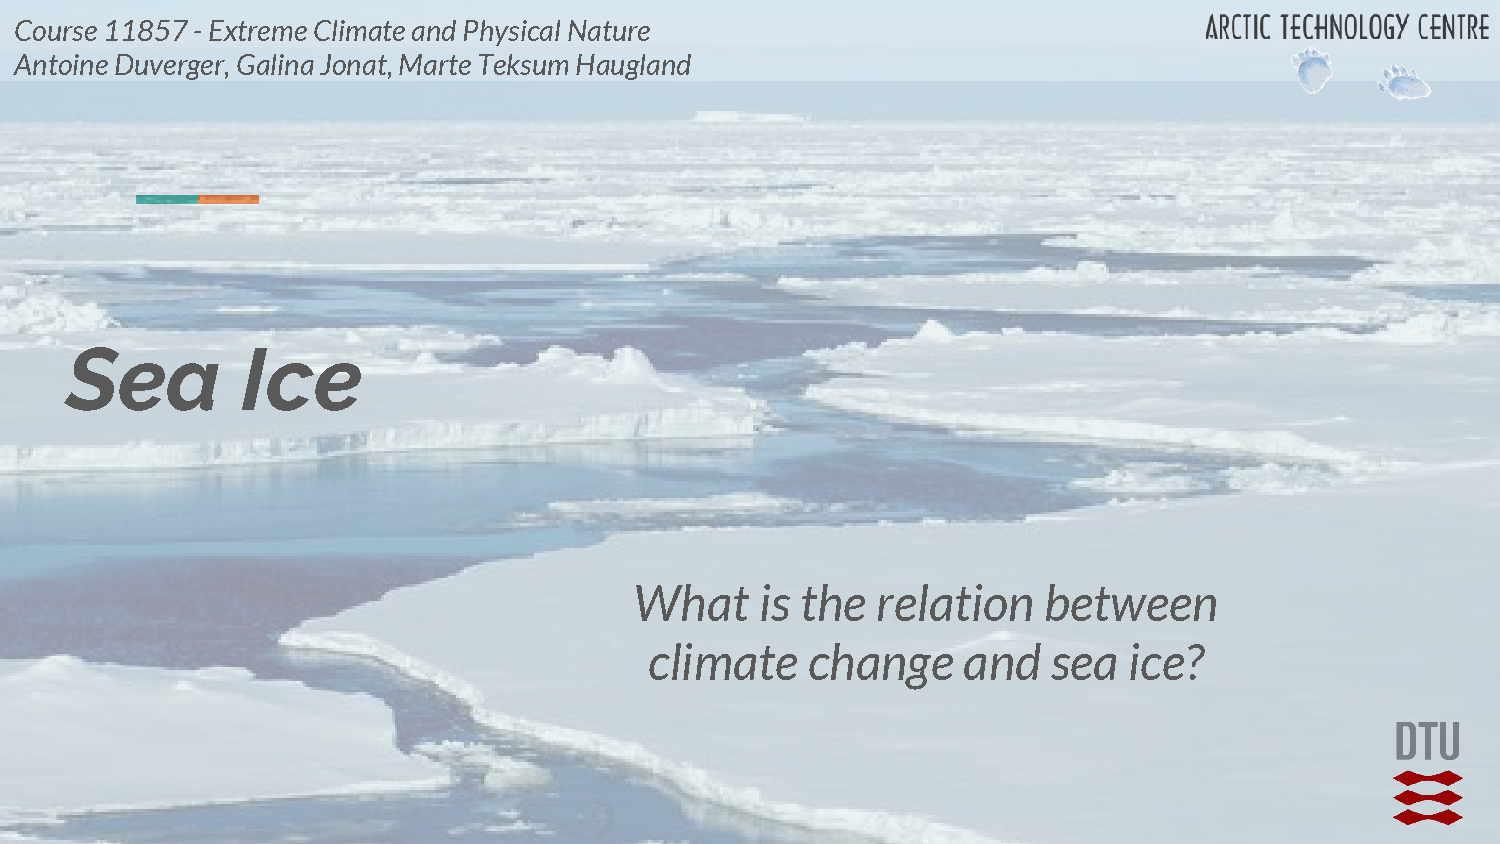
\includepdf[pages={-}, pagecommand={
                 \label{Risk_Register}}]{appendices/Sea_Ice_pres.pdf} 
    
\end{appendices}




\end{document}